\documentclass{article}

\usepackage{amsthm, amsfonts, amsmath, amssymb}
\usepackage{graphicx}
\usepackage{fullpage}

\usepackage{xcolor}
\definecolor{commentsColor}{rgb}{0.497495, 0.497587, 0.497464}
\definecolor{keywordsColor}{rgb}{0.000000, 0.000000, 0.635294}
\definecolor{stringColor}{rgb}{0.558215, 0.000000, 0.135316}
\usepackage{listings}
\lstset{ %
	backgroundcolor=\color{white},   				% choose the background color; you must add \usepackage{color} or \usepackage{xcolor}
	basicstyle=\footnotesize\ttfamily,				% the size of the fonts that are used for the code
	breakatwhitespace=false,         				% sets if automatic breaks should only happen at whitespace
	breaklines=true,                 				% sets automatic line breaking
	captionpos=b,                    				% sets the caption-position to bottom
	commentstyle=\color{commentsColor}\textit,		% comment style
	frame=tb,	                   	   				% adds a frame around the code
	keywordstyle=\color{keywordsColor}\bfseries,	% keyword style
	language=Python,                 				% the language of the code (can be overrided per snippet)
	otherkeywords={*,...},           				% if you want to add more keywords to the set
	rulecolor=\color{black},         				% if not set, the frame-color may be changed on line-breaks within not-black text (e.g. comments (green here))
	stringstyle=\color{stringColor}, 				% string literal style
	title=\lstname,                  				% show the filename of files included with \lstinputlisting; also try caption instead of title
	columns=fixed                   				% Using fixed column width (for e.g. nice alignment)
}

\usepackage{hyperref}

\newtheorem{lemma}{Lemma}
\newtheorem{theorem}{Theorem}
\newtheorem{corollary}{Corollary}
\newtheorem{conjecture}{Conjecture}
\newtheorem{definition}{Definition}

\setlength{\parindent}{0em}

\renewcommand{\O}{\mathcal{O}}
\newcommand{\xor}{\oplus}

\begin{document}
	\title{A Fast, Iterative Way to Compute Chebyshev Polynomials related to \textit{Lights Out} over GF(2)}
	\author{William Boyles}
	\date{\today}
	\maketitle
	
	\section{Introduction \& Definitions}
	\begin{definition}
		$U(n,x)$ is the degree $n$ Chebyshev polynomial of the second kind and is defined by the following recurrence relation:
		\begin{equation*}
			U(n,x) = \begin{cases}
				1 & n = 0 \\
				2x & n = 1 \\
				2x U(n-1,x) - U(n-2,x) & n \geq 2
			\end{cases}.
		\end{equation*}
	\end{definition}
	\begin{definition}
		$f(n,x)$ is $U(x/2)$ over the field $GF(2)$.
		So, it is defined by the following recurrence relation:
		\begin{equation*}
			f(n,x) = \begin{cases}
				1 & n = 0 \\
				x & n = 1 \\
				x f(n-1,x) \xor f(n-2,x) & n \geq 2
			\end{cases},
		\end{equation*}
		where $\xor$ is the addition operator over GF(2) (aka XOR).
	\end{definition}
	It's known that the nullity, $d(n)$ of an $n \times n$ \textit{Lights Out} board is the degree of $\gcd(f(n,x), f(n,x+1))$.
	So, one needs to be able to calculate $f(n,x)$ and $f(n,x+1)$ efficiently to calculate $d(n)$ efficiently.
	Ideally, the algorithm would not require calculating all of $f(0,x) \dots f(n-1,x)$ and $f(0,x+1) \dots f(n-1,x+1)$.
	We present such algorithms to calculate $f(n,x)$ and $f(n,x+1)$ in $O(n)$ and $O(n\log{n})$ time respectively, both with $O(1)$ extra space.
	
	\section{Investigating Patterns}
	\subsection{Patterns in $f(n,x)$}
	Since $f(n,x)$ is a polynomial over $GF(2)$, all of its coefficients are either 1 or 0.
	So, a sensible way to visualize $f(n,x)$ would be to color squares black or white to represent the coefficients.
	For example,
	\begin{equation*}
		f(5,x) = 1x^5 + 0x^4 + 0x^3 + 0x^2 + 1x + 0 = \blacksquare\square\square\square\square\blacksquare\square.
	\end{equation*}
	We'll also enumerate the list of in the following way:
	Let $f(n,x)_i$ be the $i$th entry in the coefficient list of $f(n,x)$ so that $f(n,x)_0$ is the highest degree term and $f(n,x)_n$ is the units term.
	So, $f(5,x)_0 = 1$, $f(5,x)_1 = 0$, and $f(5,x)_5 = 0$.
	
	If we plot out $f(0,x)$ through $f(128,x)$ in the same way, aligning terms of the same degree (the degree any square represents is $n-i$), we get the following image:
	
	\begin{center}
		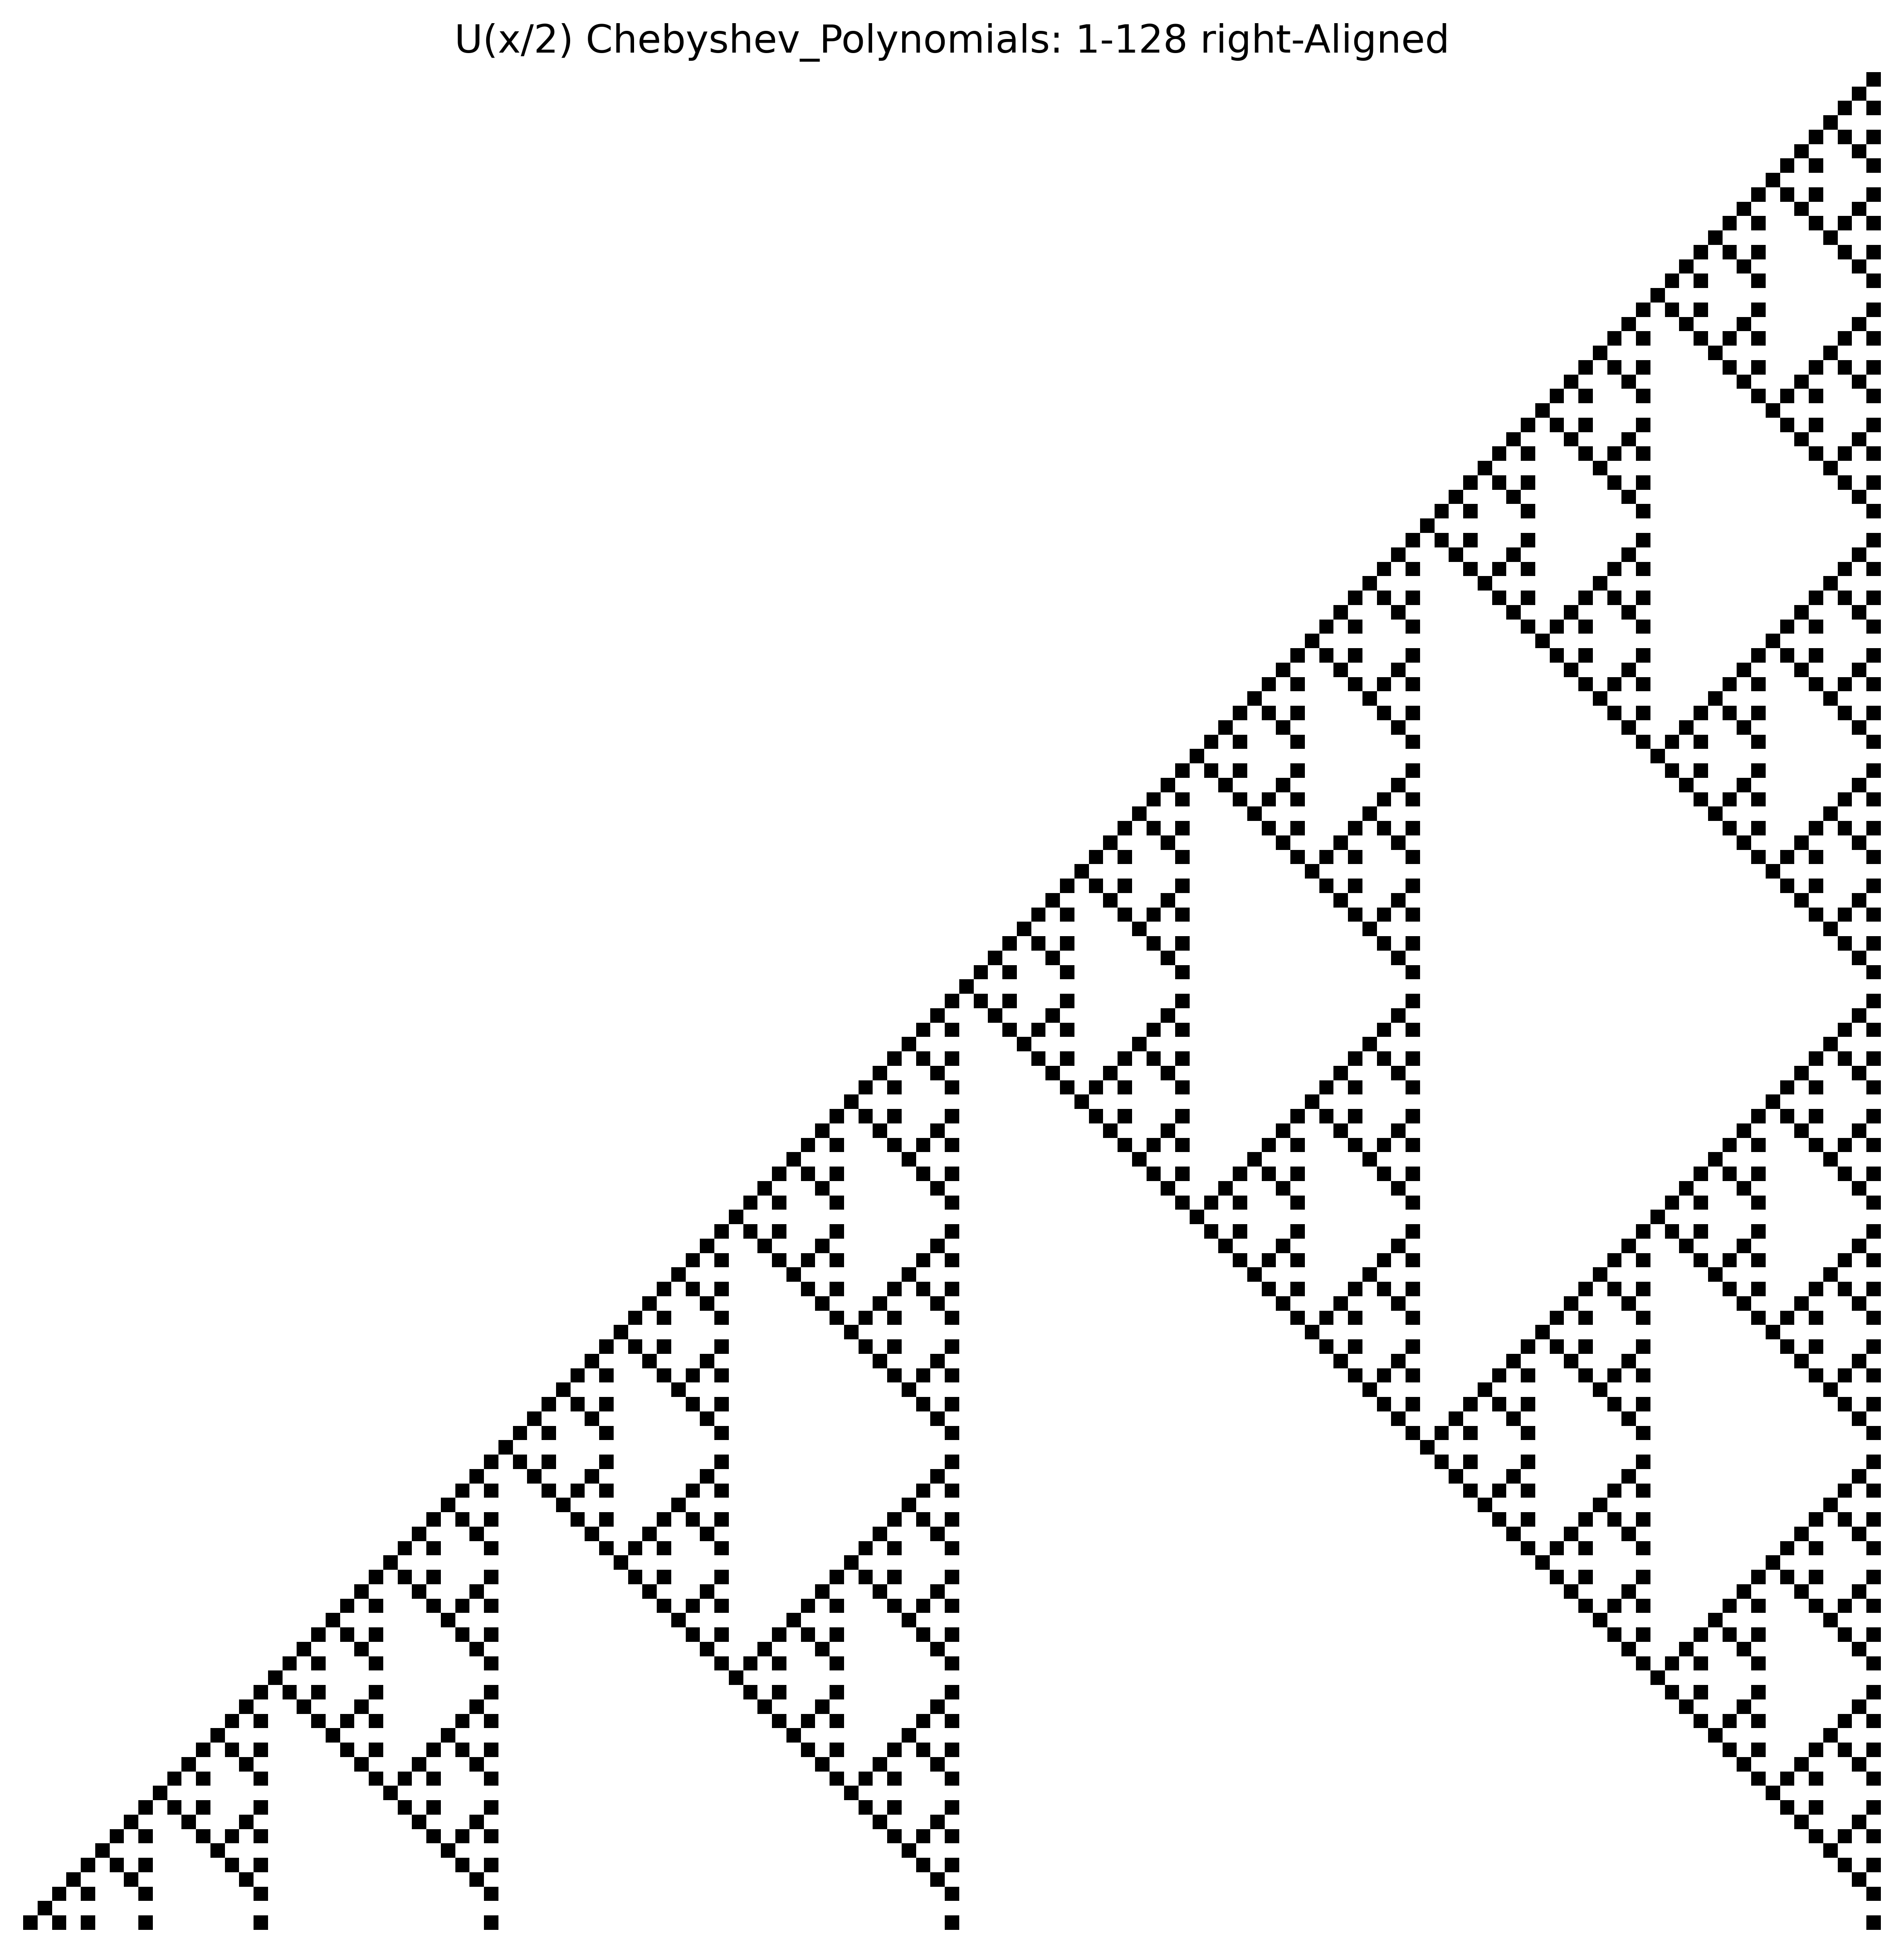
\includegraphics[width=.8\textwidth]{../../code/serialization/chebyshev/chebyshev1_right_128.png}	
	\end{center}
	
	If one is familiar with elementary cellular automaton, then they will recognize this pattern as rule 90.

	\begin{center}
		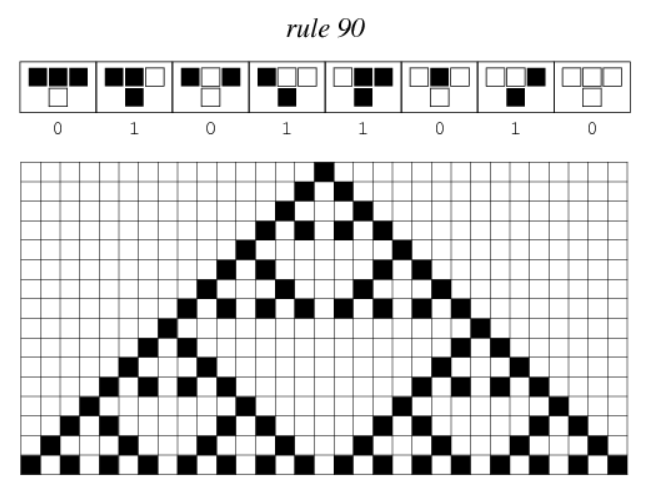
\includegraphics[width=0.8\textwidth]{rule90.png}
	\end{center}

	\begin{theorem}
		For any positive integer $k$, plotting $f(0,x)$ through $f(2^k - 1,x)$ inclusive yields the right half of rule 90. 
	\end{theorem}
	\begin{proof}
		First, note that the first two rows in our image are equal to the last two columns produced by rule 90 after $2^k - 1$ steps.
		So, for $n \leq 2$, our relationships holds.
		
		Assume $n > 2$.
		By the definitions of $f(n,x)$,
		\begin{equation*}
			f(n,x) = xf(n-1,x) \xor f(n-2,x).
		\end{equation*}
		For a particular cell,
		\begin{equation*}
			f(n,x)_i = f(n-1,x)_i \xor f(n-2)_{i-2}.
		\end{equation*}
		Rearranging,
		\begin{equation*}
			f(n-1,x)_i = f(n,x)_i \xor f(n-2)_{i-2}.
		\end{equation*}
		This is exactly what rule 90 tells us: The state of a cell in a subsequent row (column in our image) is the XOR of the two cells to the left and right in the above row, and that the cell immediately above does not affect the outcome.
	\end{proof}

	\subsection{Rule 90 and Binomial Coefficients}
	It's well-known that the value of a cell in rule 90 can be found via the parity of binomial coefficients.
	We can write this knowledge in terms of $f(n,x)$.
	
	\begin{lemma}
		Let $f(n,x)_i$ be the $i$th entry in the coefficient list of $f(n,x)$ so that $f(n,x)_0$ is the highest degree term and $f(n,x)_n$ is the units term.
		Let $K = 2^k - 1$ where $k$ is the smallest integer such that $K \geq n$.
		Let $S = 2(K-n)$.
		Then
		\begin{equation*}
			f(n,x)_i = \begin{cases}
				1 & \binom{2i + S}{S + i} \text{ is odd} \\
				0 & \text{otherwise}
			\end{cases}.
		\end{equation*}	
	\end{lemma}

	So, we just need a quick way to calculate the parity of binomial coefficients.
	

	Here's a neat fact about the divisibility of binomial coefficients.
	
	\begin{theorem}[Kummer's Theorem]
		Let $p$ be a prime, $n$ and $m$ positive integers.
		Then the highest power of $p$ that divides $\binom{n+m}{m}$ is the number of carry operations when adding $n$ and $m$ in base $p$.
	\end{theorem}
	
	Since we're concerned with base 2, we can give a more specific version of this result.
	
	\begin{corollary}
		$\binom{n+m}{m}$ is odd if and only if the bitwise AND of $n$ and $m$, is 0.
	\end{corollary}
	
	\subsection{Patterns in $f(n,x+1)$}
	$f(n,x+1)$ is also a polynomial over $GF(2)$, so all of its coefficients are 1 or 0.
	So, we can visualize it in the same way we did for $f(n,x)$.
	For example,
	\begin{equation*}
		f(5,x+1) = 1x^5 + 1x^4 + 0x^3 + 0x^2 + 0x + 0 = \blacksquare\blacksquare\square\square\square\square.
	\end{equation*}
	Plotting $f(0,x+1)$ through $f(128,x+1)$ in the same way, aligning terms of the same degree, we get the following image.
	
	\begin{center}
		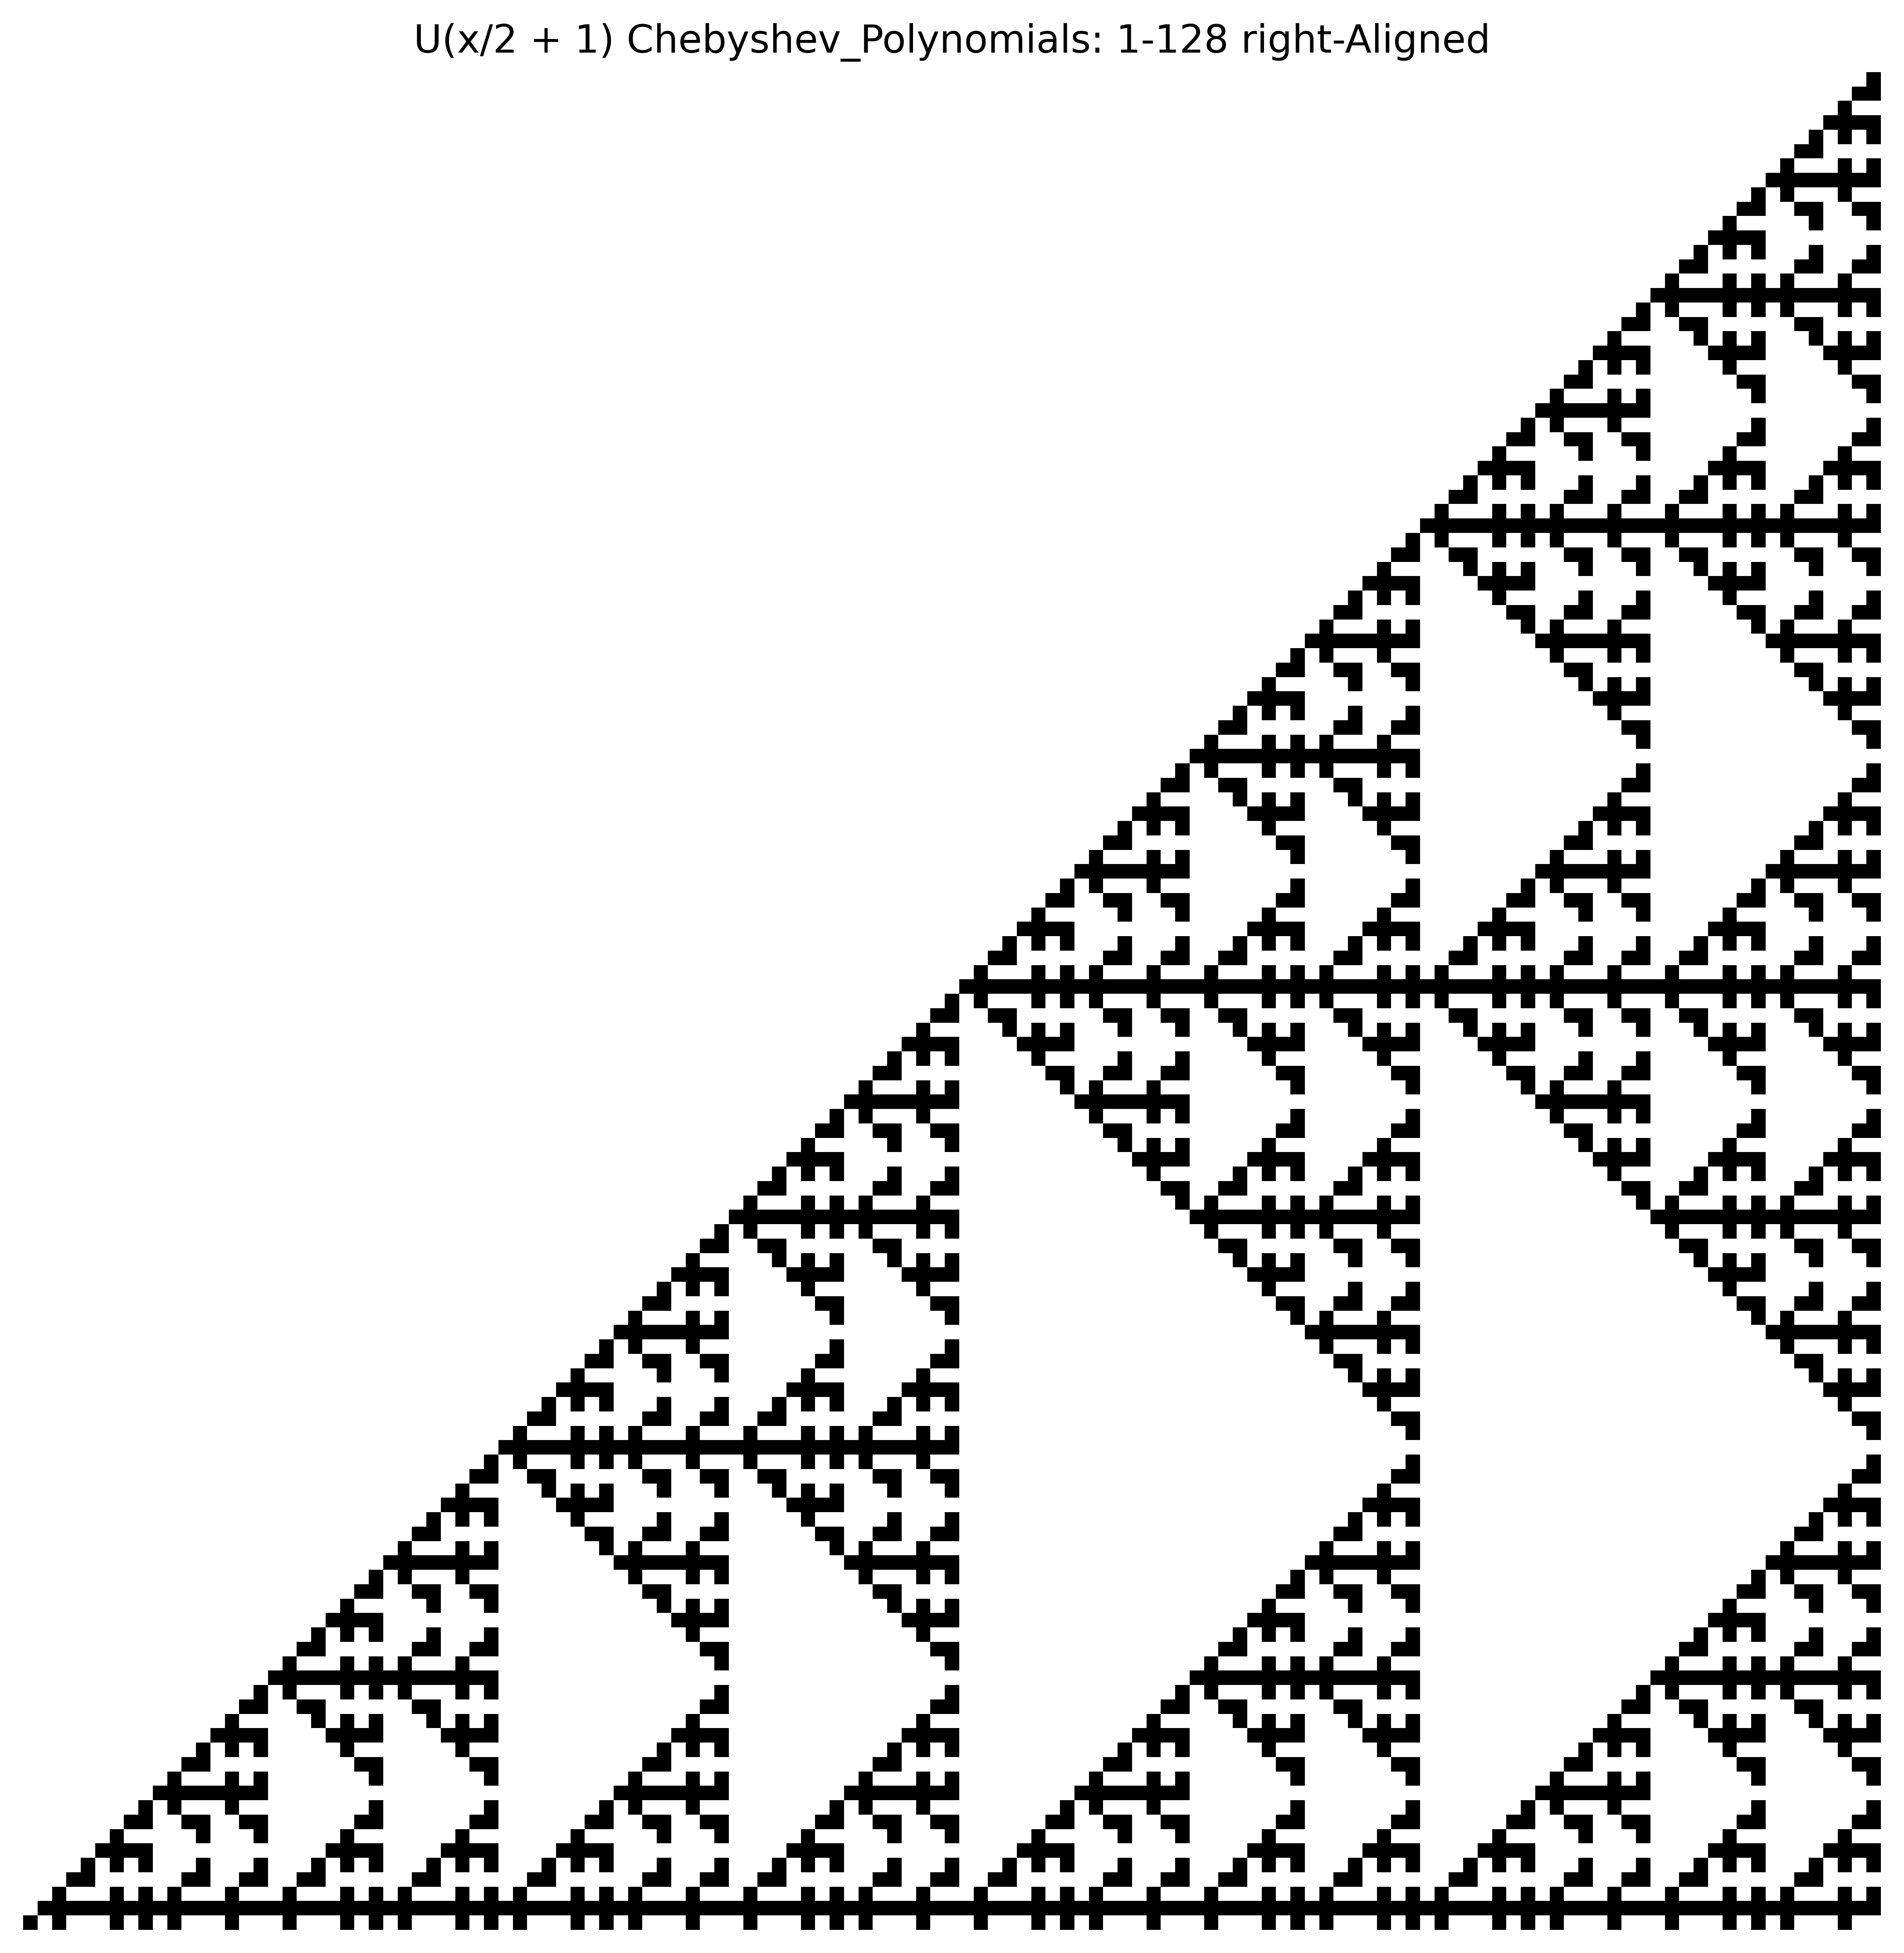
\includegraphics[width=.8\textwidth]{../../code/serialization/chebyshev/chebyshev2_right_128.png}	
	\end{center}

	Again, if one is familiar with elementary cellular automaton, then they will recognize this pattern as rule 150.
	
	\begin{center}
		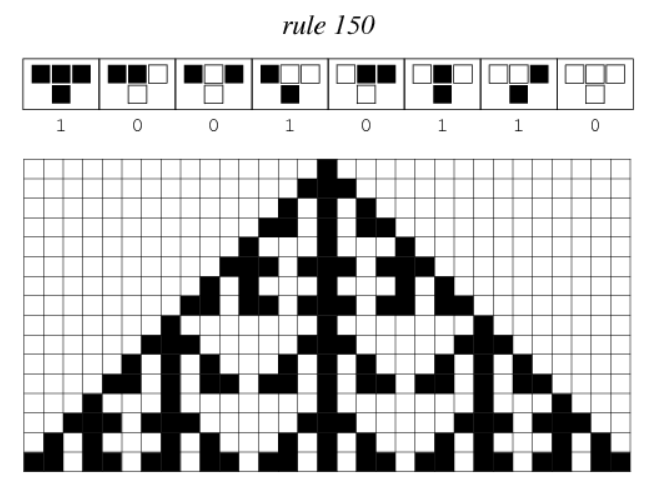
\includegraphics[width=0.8\textwidth]{rule150.png}
	\end{center}

	\begin{theorem}
		For any positive integer $k$, plotting $f(0,x+1)$ through $f(2^n - 1,x+1)$ inclusive, yields the right half of rule 150.
	\end{theorem}
	\begin{proof}
		We will prove that our rule for determining a value of a certain ``cell'' in the image above is equivalent to rule 150.
		
		First, note that the first two rows in our image are equal to the last two columns produced by rule 150 after $2^k - 1$ steps.
		So, for $n \leq 2$, our relationship holds.
		
		Assume $n > 2$.
		By the definition of $f(n,x+1)$,
		\begin{align*}
			f(n,x+1) &= (x+1)f(n-1,x+1) \xor f(n-2,x+1) \\
			&= xf(n-1,x+1) \xor f(n-1,x+1) \xor f(n-2,x+1).
		\end{align*}
		For a particular cell,
		\begin{equation*}
			f(n,x+1)_i = f(n-1,x+1)_i \xor f(n-1,x+1)_{i-1} \xor f(n-2,x+1)_{i-2}.
		\end{equation*}
		Rearranging,
		\begin{equation*}
			f(n-1,x+1)_{i-1}  = f(n,x+1)_{i} \xor f(n-1,x+1)_{i} \xor f(n-2,x+1)_{i-2}.
		\end{equation*}
		This is exactly what rule 150 tells us: The state of a cell in a subsequent row (column in our image) is the XOR of the three closest above cells in the previous row.
	\end{proof}
	
	
	\subsection{Rule 150 and Trinomial Coefficients}
	Much like how one can obtain the pattern formed by rule 90 from odd numbers in the triangle of binomial coefficients (i.e. Pascal's Triangle), one can obtain the pattern formed by rule 150 from odd numbers in the triangle of trinomial coefficients known as the Trinomial Triangle, where each subsequent row has 2 more entries than the previous.
	
	\begin{definition}
		The trinomial coefficient in the $n$th row and $k$th column of the trinomial triangle, $\binom{n}{k}_2$ is defined by the following relationships:
		\begin{equation*}
			\binom{n}{k}_2 = \begin{cases}
				0 & k < 0 \text{ or } k > 2n + 1 \\
				0 & n < 0 \\
				1 & k = 0 \text{ and } n = 0 \\
				\binom{n-1}{k-1}_2 + \binom{n-1}{k}_2 + \binom{n-1}{k+1}_2 & \text{otherwise}
			\end{cases}.
		\end{equation*}
	\end{definition}

	Note the similarity in the definition to that of rule 150. \\

	Here's another fact similar to Kummer's Theorem about the divisibility of binomial coefficients.
	\begin{theorem}[Lucas's Theorem]
		Let $p$ be a prime, $n$ and $m$ positive integers.
		The the following congruence relation holds:
		\begin{equation*}
			\binom{m}{n} = \prod_{i=0}^{k}{\binom{m_i}{n_i}} \mod p,
		\end{equation*}
		where
		\begin{align*}
			m &= m_kp^k + m_{k-1}p^{k-1} + \dots + m_1p + m_0 \\
			n &= n_kp^k + n_{k-1}p^{k-1} + \dots + n_1p + n_0,
		\end{align*}
		the base $p$ expansion of $m$ and $n$ respectively.
	\end{theorem}

	\begin{corollary}
		TODO: I don't really understand what's going on in this answer, but it provides us with an algorithm for the parity of a trinomial in $\O(log n)$ time. \\
		
		\href{https://stackoverflow.com/a/43698262}{https://stackoverflow.com/a/43698262} gives us the trinomial analog for $p=2$.
	\end{corollary}

	\section{The Algorithms}
	\subsection{Algorithm for $f(n,x)$}
	Putting all the pieces together, here is the algorithm to calculate the coefficient list of $f(n,x)$.
	
	\begin{center}
	\begin{verbatim}
	from math import ceil, log2
		
	def binomial_parity(n: int, m: int) -> int:
	    return 0 if ((n-m) & m) else 1
		
	def f(n: int) -> list[int]:
	    K = (1 << ceil(log2(n + 1))) - 1
	    S = 2*(K - n)
	    
	    return [binomial_parity(2*i + S, i + S) for i in range(n+1)]
	\end{verbatim}
	\end{center}

	To compute \texttt{f(n)}, this algorithm makes $\O(n)$ calls to \texttt{binomial\_parity}.
	Assuming operations like comparison, subtraction, and bitwise AND between 2 integers takes $\O(1)$ time, computing \texttt{f(n)} takes $\O(n)$ time.

	\subsection{Algorithm for $f(n,x+1)$}
	Putting all the pieces together, there is the algorithm to calculate the coefficient list of $f(n,x+1)$.
	
	\begin{center}
	\begin{verbatim}
	from math import ceil, log2
	
	def trinomial_parity(n: int, m: int) -> int:
	    a, b = 1, 0
	    while m:
        	n1, n = n & 1, n >> 1
        	m1, m = m & 1, m >> 1
        	a, b = ((n1 | ~m1) & a) ^ (m1 & b), ((n1 & ~m1) & a) ^ (n1 & b)
	    
	    return a
	    
	def f2(n: int) -> list[int]:
	    K = (1 << ceil(log2(n + 1))) - 1
	    S = K - n
	    
	    return [trinomial_parity(S + i, 2*S + i) for i in range(n+1)]
	\end{verbatim}
	\end{center}

	To compute \texttt{f2(n)}, this algorithm makes $\O(n)$ calls to \texttt{trinomial\_parity}.
	Each iteration of the while loop in \texttt{trinomial\_parity} halves \texttt{m}, so \texttt{trinomial\_parity} runs in $\O(\log{m})$ time.
	The \texttt{m} parameter passed in by \texttt{f2} is $\O(n)$, so each call to \texttt{trinomial\_parity} in \texttt{f2} takes $O(\log{n})$ time.
	So, \texttt{f2(n)} runs in $O(n\log{n})$ time.
\end{document}